% UICTEST.TEX
% This is a test file for my port of UICTHESI
% to LaTeX 2e. This is based in part on UCTHESIS.
%

\documentclass{uicthesi}




\usepackage{booktabs} % For formal tables

\usepackage{framed}
\usepackage{hyperref}
\usepackage{balance}
\usepackage[dvips]{graphics,color}
\usepackage{tabularx}

\usepackage{epsfig}
\usepackage{color}
\usepackage{subfigure}
\usepackage{multirow,tabularx}
\usepackage{placeins}
%\usepackage{miniltx}
\usepackage{mathtools}
\usepackage{graphicx}
\usepackage{epstopdf}
\usepackage{bm}

\usepackage{csquotes}
\usepackage{array}
\usepackage[yyyymmdd,hhmmss]{datetime}
\usepackage[subject={Todo}]{pdfcomment}
\usepackage[textsize=scriptsize,bordercolor=black!20]{todonotes}
\usepackage{xcolor,colortbl}
\usepackage{amssymb}% http://ctan.org/pkg/amssymb
\usepackage{pifont}% http://ctan.org/pkg/pifont
\usepackage[algo2e,titlenumbered,ruled]{algorithm2e} 
\usepackage{lipsum,environ,amsmath}
\usepackage{slashbox,booktabs,amsmath}
%\usepackage{todonotes}
\usepackage{cite}

\usepackage{xspace}

\hyphenation{PageRank Convex dictatorship Dic-ta-tor-ship}

\newcounter{Lcount}
\newcommand{\numsquishlist}{
   \begin{list}{\arabic{Lcount}. }
    { \usecounter{Lcount}
 \setlength{\itemsep}{-.1ex}      \setlength{\parsep}{0ex}
      \setlength{\topsep}{0ex}       \setlength{\partopsep}{0ex}
      \setlength{\leftmargin}{1em} \setlength{\labelwidth}{1em}
      \setlength{\labelsep}{0.1em} } }
\newcommand{\numsquishend}{\end{list}}

\newcommand{\squishlist}{
   \begin{list}{$\bullet$}
    { \setlength{\itemsep}{-.1ex}      \setlength{\parsep}{0ex}
      \setlength{\topsep}{0ex}       \setlength{\partopsep}{0ex}
      \setlength{\leftmargin}{.8em} \setlength{\labelwidth}{1em}
      \setlength{\labelsep}{0.5em} } }
\newcommand{\squishend}{\end{list}}



\makeatletter
\DeclareOldFontCommand{\rm}{\normalfont\rmfamily}{\mathrm}
\DeclareOldFontCommand{\sf}{\normalfont\sffamily}{\mathsf}
\DeclareOldFontCommand{\tt}{\normalfont\ttfamily}{\mathtt}
\DeclareOldFontCommand{\bf}{\normalfont\bfseries}{\mathbf}
\DeclareOldFontCommand{\it}{\normalfont\itshape}{\mathit}
\DeclareOldFontCommand{\sl}{\normalfont\slshape}{\@nomath\sl}
\DeclareOldFontCommand{\sc}{\normalfont\scshape}{\@nomath\sc}
\makeatother


\newcounter{problem}
\newenvironment{problem}[1][htb]
  {\renewcommand{\algorithmcfname}{Problem}% Update algorithm name
   \begin{algorithm2e}[#1]%
   \SetAlFnt{\small}
    \SetAlCapFnt{\small}
    \SetAlCapNameFnt{\small}
    \SetAlCapHSkip{0pt}
  }{\end{algorithm2e}}
  
  \newenvironment{alprocedure}[1][htb]
  {\renewcommand{\algorithmcfname}{Procedure}% Update algorithm name
   \begin{algorithm2e}[#1]%
    \SetAlFnt{\small}
\SetAlCapFnt{\small}
\SetAlCapNameFnt{\small}
\SetAlCapHSkip{0pt}
\IncMargin{-\parindent}
   
  }{\end{algorithm2e}}
  


\begin{document}

% Declarations for Front Matter

\title{Asynchronous Delegation and its Applications}
\author{George Dill}
\pdegrees{BSc (Purdue University, West Lafayette, IN) 2008}
\degree{Master of Science in Computer Science}
\committee{Prof. Jakob Eriksson, Chair and Advisor \\ Prof. Xingbo Wu  \\ Prof. William Mansky \\ }
\maketitle


% \dedication
% {\null\vfil
% {\large
% \begin{center}
% To myself,\\\vspace{12pt}
% Perry H. Disdainful,\\\vspace{12pt}
% the only person worthy of my company.
% \end{center}}
% \vfil\null}


 \acknowledgements
{The thesis has been completed... (INSERT YOUR TEXTS)\\ 

\begin{flushright}YOUR INITIAL\end{flushright}}
% \acknowledgements
% {I want to ``thank'' my committee, without whose ridiculous demands, I
% would have graduated so, so, very much faster.}

% \preface
% This preface is purely optional at UIC.

\preface


\tableofcontents
\listoftables
\listoffigures
\listofabbreviations
\begin{list}
{}
{\setlength
  {\labelwidth}{1in}
    \setlength{\leftmargin}{1.5in}
    \setlength{\labelsep}{.5in}
    \setlength{\rightmargin}{\leftmargin}}
\item[AMS\hfill] American Mathematical Society
\item[CPU\hfill] Central Processing Unit
\item[CTAN\hfill] Comprehensive \TeX\ Archive Network
\item[FFWD\hfill] Fast, Flyweight Delegation
\item[FIFO\hfill] First In First Out
\item[KB\hfill]  $2^{10}$ Bytes
\item[MOPS\hfill] Million Operations per Second
\item[NUMA\hfill] Non Uniform Memory Access
\item[TUG\hfill] \TeX\ Users Group
\item[UIC\hfill] University of Illinois at Chicago
\item[UICTHESI\hfill] Thesis formatting system for use at UIC.
\end{list}
 
\summary
Synchronization by delegation has been shown to increase total throughput in highly parallel systems over coarse grained locking, \cite{ffwd} but the latency inherent in passing messages between cores introduces a bottleneck in overall throughput. To mitigate the effects of this bottleneck we introduce parallelism in message passing by enabling asynchronous delegation calls. 

We present an asynchronous design for both dedicated and flat delegation strategies. In dedicated delegation hardware threads act exclusively as a client or server as opposed to flat delegation where hardware threads share duty as both client and server. 

This work is based upon \textit{Gepard} which provides parallelism by using fibers, a user space threading library. Our asynchronous approach removes the memory and computation overhead of switching between fibers, freeing cache resources and processor cycles. Even more concurrency in message passing is added to the \textit{Gepard} server design by increasing the number of requests lines per server from 4 to 16. The result is a throughput increase of up to 400 MOPS on our test bench.  

We compare the designs and throughput of asynchronous delegation to that of Gepard \cite{gepard}, fine grained locks, and atomic operations on a fetch and add microbenchmark. We find that dedicated asynchronous delegation outperforms all other synchronization schemes tested when the delegated data structure remains in the server's cache. Flat delegation performs comparably to fine grained locking approaches for very large shared data structures where DRAM access latency dominates performance. 

\chapter{Background and Motivation}
\section{Synchronization}
Parallel programs traditionally follow a model where multiple threads perform operations on the same data structure. This model creates the opportunity for a simultaneous access of shared memory by multiple threads that yields a non-deterministic result, or data race. The commonly implemented solution is to synchronize access to shared data structures through mutual exclusion (mutex) locks. 

Mutex locks are realized through the use of locked atomic instructions. For access to individual words, locked atomic instructions provide a guarantee that a write will be seen consistently across all threads. The guarantee can be made by locking the system bus, but is more often achieved through the processor's cache coherency policy \cite{IntelDevelopersManual}. The locked operations are slower than their standard counterparts; for example the locked compare and exchange instruction, LOCK CMPXCHG, on Intel Skylake takes 18 cycles while a CMPXCHG  instruction takes 6 \cite{agner}. 

A mutex lock works by 'claiming' a variable using an atomic instruction like LOCK CMPXCHG. If a thread is successful in writing to the variable it can proceed to operate on the critical section of shared memory, and then release the lock. If the thread is unsuccessful it will wait by some policy until it successfully claims the lock variable. This programming pattern serializes accesses to the shared memory therefore eliminating the data race. However when a lock is contended, threads may spend an inordinate amount of time waiting to acquire the lock rather than performing useful calculations. 

\section{Delegation}
\begin{figure}[ht!]
\centering
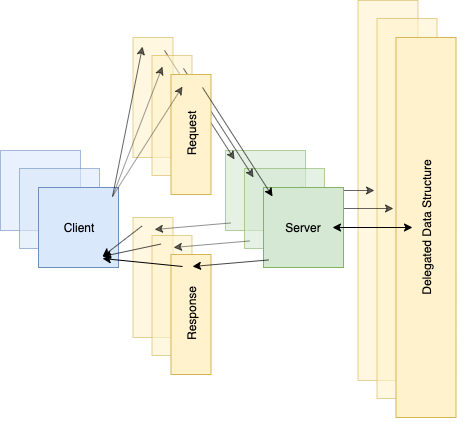
\includegraphics[width=0.9\columnwidth]{FIG/general_delegation.png}
\caption{A delegation system with 3 clients and 3 servers. The foreground client makes a request to all three servers. }
\label{fig:general_delegation}
\end{figure}
Delegation, as described by Roghanchi et. al. in \textit{FFWD}\cite{FFWD}, grants exclusive control of a data structure to a single thread called a \textit{server}. \textit{Client} threads delegate operations on data structures to the appropriate \textit{server} by passing a message called a request. The \textit{server} is one thread, performing one operation at a time. The delegated operations are serialized and the data race eliminated. 

In \textit{FFWD} style delegation, servers receive requests to perform an operation on their memory from \textit{clients} via a 64 Byte struct containing a function pointer, up to 6 arguments, and a status flag. Similarly, responses are communicated via a 16 Byte struct containing a return value and a status flag.  

Every server-client pair has at least one dedicated request line and one dedicated response line. ~\ref{fig:general_delegation} shows a system with 3 clients and 3 servers. The client in the foreground makes a request to its allocated request line on all three servers. The server performs an operation on its delegated data structure, and writes the response to the response line allocated to that specific client. Since each request and response line has only one writer, there is no data race nor any cache line contention.

Each delegation \textit{server} iterates through an array of requests. When a new request is encountered, the server loads the requested parameter values into the appropriate registers and then calls the function pointer. The server stores the return value from the function and the flag variable into the corresponding index in the array of responses.  

Programs using the delegation library typically initialize the data structure to delegate, launch the dedicated servers, and then launch threads running the client function through a POSIX threads like interface. 

An advantage of delegation is spatial locality of memory. A block of memory accessed exclusively by a delegation server is never shared with another thread. A small delegated data structure may fit within a server's on-core cache and remain resident for the duration of the program. In contrast, a system with multiple physical cores accessing the same data structure will share cache lines, greatly reducing the likelihood of a high level cache hit. 

From the client perspective, a drawback of delegation is the latency from request issuance to response. In \textit{FFWD}, a synchronous delegation system, clients issue a request to the server's request line and then poll the respective response line until the request is returned. The time to complete a single delegated operation includes the time to write to the server, perform the function, and then receive the response. 

\textit{Gepard} introduces concurrency in delegation operations while maintaining a synchronous interface by enabling a thread to switch to productive work through the use of fibers. Based upon \textit{libfiber} \cite{libfiber}, \textit{Gepard} fibers are light-weight, cooperatively scheduled user mode threads. \textit{Gepard} threads run a fiber manager overseeing multiple client fibers. A client fiber writes a delegation request to the server then yields, thereby invoking the fiber manager which switches context to another client fiber. After some time the original client fiber will be reactivated and continue execution. The major advantage of \textit{Gepard} is that it enables a single thread to engage with multiple servers concurrently with the effect of increasing throughput despite constant individual request latency. 

\chapter{Asynchronous Delegation}

\begin{table}[ht!]
\begin{tabularx}{\linewidth}{| r | X |} %{ | p{2.5 in} p{4 in} | }
  \hline
  \bf{Function} & \bf{Description} \\
  \hline
  \bf{Launch\_Servers(n)} & Starts the specified number of server threads, allocates and initializes the request and response lines. \\
  \hline
  \bf{Client\_Thread\_Create(f, arg)} & Allocates and initializes a pending request queue for every server as thread local variable. Launches an OS thread to run function f with argument arg. \\
  \hline
  \bf{Delegate\_Async(s, cb, f, args...)} & Generates a delegation request to server s with function f and arguments args. Calls cb with the return value from f. \\
  \hline
  \bf{Async\_Barrier()} & Places requests from a delegated thread's queue and polls server responses until all requests have been served. \\
  \hline
\end{tabularx}
\label{tab:api}
\caption{Excerpt of the asynchronous delegation API}
\end{table}

By decoupling a delegation call from its response, asynchronous delegation is able to introduce more concurrency than \textit{Gepard} and achieve greater system throughput. Operations which \textit{Gepard} performs after a call to \textbf{delegate(s, retval, f, args)} are now done in a callback function invoked upon receipt of the response. The callback, if required, is passed to the delegate function in place of the return value as shown by \textbf{Delegate\_Async(s, cb, f, args)}. An excerpt of the asynchronous delegation API is shown  in ~\ref{tab:api}. 

The change in API allows asynchronous delegation to completely remove \textit{libfiber}, the agent of client side concurrency in \textit{Gepard}, along with \textit{libfiber's} associated memory and computation overhead. \textit{Gepard} fiber managers keep track of a fiber's state which includes its call stack and instruction pointer. In contrast, asynchronous delegation tracks a client's request leaving the restoration of state to the callback function. By a combination of memory footprint and compuation overhead in contexting switching, \textit{Gepard's} throughput peaks at 64 fibers / thread. On the other hand, we show asynchronous delegation efficiently tracks well over 1,000 concurrent, outstanding pending requests in our benchmarks. 

The reserve of pending requests is available because calls to \textbf{Delegate\_Async()} are non-blocking for most invocations. The client function can continue to generate requests while interaction with the delegation server is deferred until the most optimal time depending on the delegation strategy. 

In this chapter we explore the opportunities that this explosion of available requests provides to increase concurrency in asynchronous delegation with one or more dedicated server threads. Later, we show how asynchronous operation can be applied to flat delegation, a more recent, serverless design. 

Figures in this chapter are generated with variations of a fetch and add benchmark. In this benchmark (1ea) 64B, variable is allocated for each delegation server in the system. For a period of three seconds, clients select a server at random and delegate an increment function to the server. The function increments the server's variable and returns. There is no callback. Results shown are the harmonic mean of ten samples. Unless otherwise stated, asynchronous delegation is configured with 16 request lines per client - server pair and a 32 length pending request queue for each server.  

\section{Asynchronous Dedicated Delegation}
\begin{figure}[ht!]
\centering
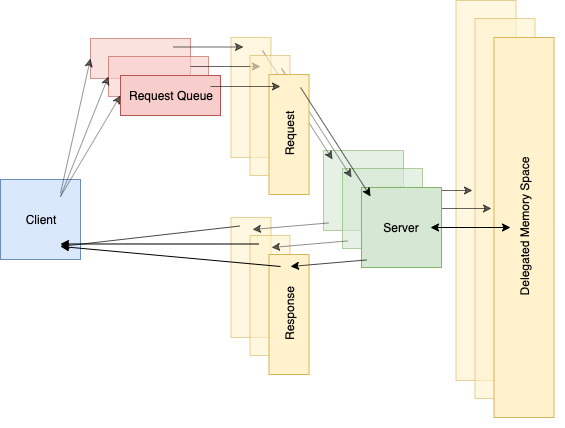
\includegraphics[width=0.9\columnwidth]{FIG/dedicated_async.png}
\caption{An asynchronous delegation system with 1 client and 3 servers in our highest throughput configuration. The foreground client makes a request to all three servers. Requests are written to a pending request queue which is periodically flushed out to the request line. }
\label{fig:dedicated_delegation}
\end{figure}

~\ref{fig:dedicated_delegation} sketches an asynchronous dedicated delegation system with 1 client and 3 servers. The client generates requests and places them in the fixed-length request queue for the required server. When any of the queues reaches capacity, the client suspends request generation and begins the process of writing out requests to servers. The client polls its response lines one by one, executing the callback function if provided. When a response is present a request is popped from the request queue and placed in the corresponding request line. After all response-request lines have been handled \textbf{Delegate\_Async()} returns. 

To use asynchronous dedicated delegation as shown in ~\ref{fig:dedicated_delegation}, the user first initializes a number of delegation servers using \textbf{Launch\_Servers}. Running on separate OS threads, the servers begin sequentially polling their request lines. The user then launches OS threads with the application code by calling \textbf{Client\_Thread\_Create}. The thread launched by \textbf{Client\_Thread\_Create} first initializes an empty queue of pending requests for each running server on the NUMA node which the client thread is assigned. After queue initialization the thread invokes the client function. 

Within the client function the programmer uses \textbf{Delegate\_Async} to delegate the request. Typically \textbf{Delegate\_Async} will enqueue the request locally and then return to the client function. However, a push to the pending request will fail when the queue is full. At this time the client iterates through its entire array of responses. If a response is ready, the client invokes the callback with the corresponding return value, and then writes a new request, popped from the appropriate pending request queue, to the corresponding request line. 

At any time the user can call \textbf{Async\_Barrier} to ensure that all pending requests are served before moving on.  \textbf{Async\_Barrier} is always called after the return of the client function and before joining the client thread. 

\subsection{Hurry Up and Wait - The Pending Request Queue} \label{pr}
\begin{figure}[ht!]
\centering
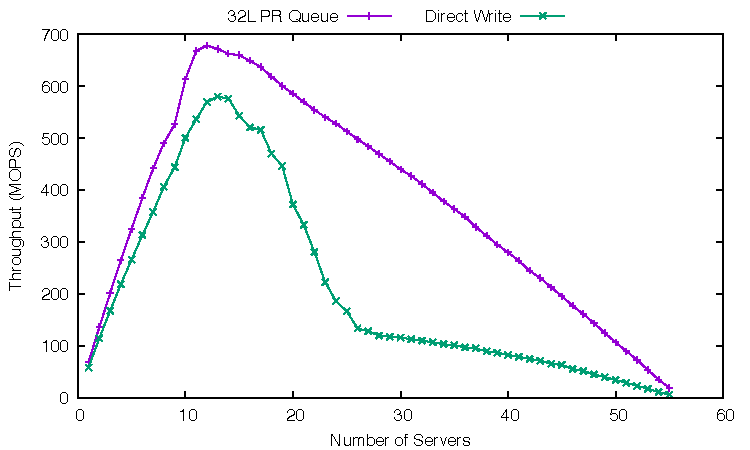
\includegraphics[width=0.9\columnwidth]{FIG/queue_v_no_queue.pdf}
\caption{Throughput in MOPS for a 56 thread system by number of servers with a 32 length pending request queue and direct request line writes.}
\label{fig:queue_v_no_queue}
\end{figure}

A counter-intuitive feature of the asynchronous API is the ability to hold a large number of pending requests in reserve until the optimal time to write them to the server. One might expect writing requests as quickly as possible to a constantly cycling server would yield the maximum throughput. However, \ref{fig:queue_v_no_queue} provides empirical evidence the reserve has a profound impact on overall system throughput. 

The experiment shown in \ref{fig:queue_v_no_queue} plots the throughput of our benchmark with a reserve queue and an asynchronous dedicated delegation configuration with direct writes to the server's request line. The direct write program tracks the index of the last request written to each server, writing its current request to the next available index. If the next index is not available the program polls the response line until it is available. Although direct write achieves comparable server consumption rate to the program with pending request reserve, it shows undesirable degradation in performance when the number of clients bounds the throughput of the system. 

We implement the request reserve as an array of pending request queues. For each client, a FIFO queue of fixed length, implemented as a circular buffer, is allocated for each server. Each call to \textbf{Delegate\_Async()} attempts to push a request onto the queue. When a push request fails, \textbf{Delegate\_Async()} iterates through its response and request lines, calling the callback on responses and writing requests from the pending request queue to the server if available. 

\begin{figure}[ht!]
\centering
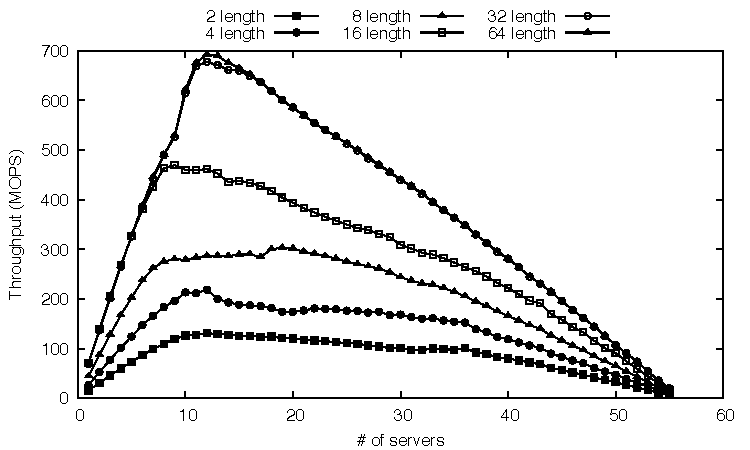
\includegraphics[width=0.9\columnwidth]{FIG/vary_queue_length.pdf}
\caption{Throughput in MOPS for a 56 thread system by number of servers by pending request queue length. The remainder of threads are clients.}
\label{fig:dedicated_vary_queue}
\end{figure}

\begin{figure}[ht!]
\centering
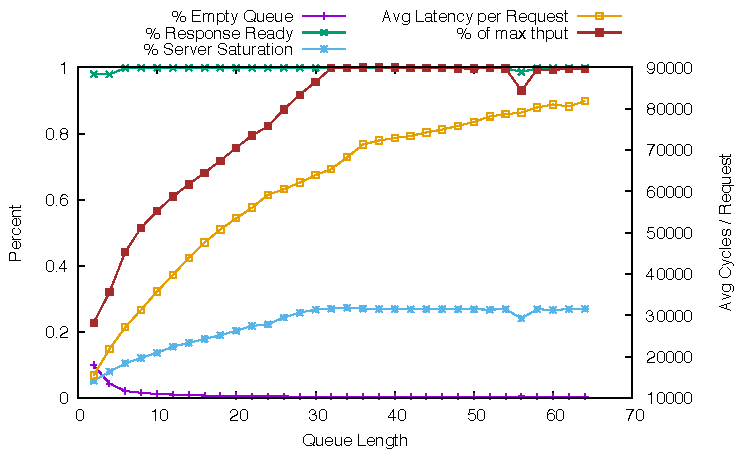
\includegraphics[width=0.9\columnwidth]{FIG/16rldedicated_saturation.pdf}
\caption{16 Request Line Configuration: Latency, Server Saturation, Response Readiness, and Failed Queue Pops by queue length.}
\label{fig:saturation16RL}
\end{figure}

\begin{figure}[ht!]
\centering
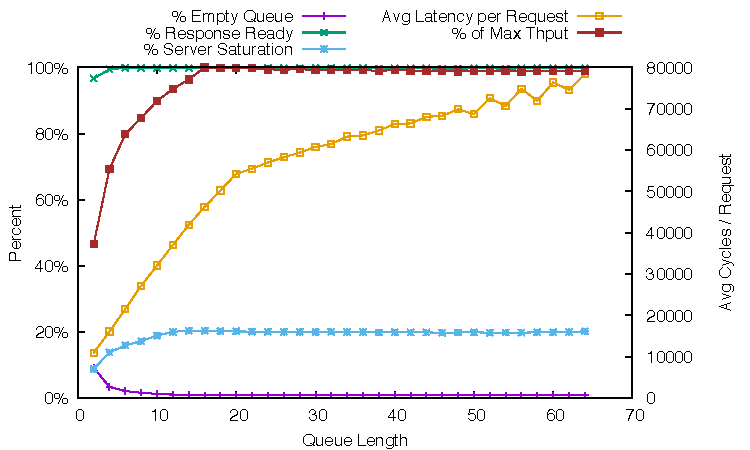
\includegraphics[width=0.9\columnwidth]{FIG/8rldedicated_saturation.pdf}
\caption{8 Request Line Configuration: Latency, Server Saturation, Response Readiness, and Failed Queue Pops by queue length.}
\label{fig:saturation8RL}
\end{figure}

\begin{figure}[ht!]
\centering
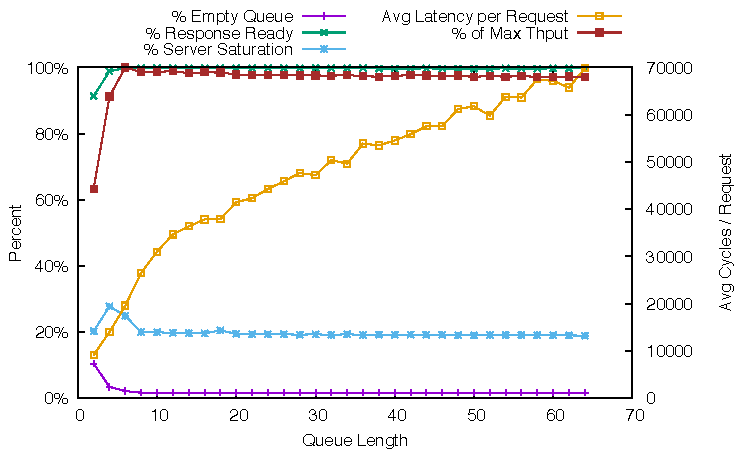
\includegraphics[width=0.9\columnwidth]{FIG/4rldedicated_saturation.pdf}
\caption{4 Request Line Configuration: Latency, Server Saturation, Response Readiness, and Failed Queue Pops by queue length.}
\label{fig:saturation4RL}
\end{figure}

How long should the individual pending request queues be? From~\ref{fig:dedicated_vary_queue} we see that the length of the pending request queue has a clear impact on overall throughput. ~\ref{fig:dedicated_vary_queue} shows our familiar benchmark plotted with various pending request queue lengths from length 2 to length 64 on a asynchronous dedicated delegation configured with 16 request lines. 2 - 8 length queues exhibit poor performance because queues smaller than the number of request lines are unable to utilize the entire capacity of the server. 

Interestingly,~\ref{fig:dedicated_vary_queue} shows that queue lengths greater than or equal to 16 show the same client consumption rate when the system is bound by server capacity; suggesting higher server saturation increases server throughput.  This relationship is confirmed by \ref{fig:saturation16RL}. \ref{fig:saturation16RL} plots throughput, server saturation, response ready rate, proportion of failed pending request queue pop operations, and average request latency with our microbenchmark using 16 servers and 40 clients. We see that peak system throughput is correlated with peak server saturation. 

From \ref{fig:dedicated_vary_queue} we also observe the marginal return on throughput for longer queue lengths diminishes after length 32, or $2 * N_{request lines}$. For more insight into this, we again reference ~\ref{fig:saturation16RL}. Server saturation increases and failed queue pop instances decrease with the extension of the pending request queue. At roughly $2 * N_{request lines}$ the gains cease. This finding suggests that the probability of having enough requests in all queues to fill all request lines approaches 1 somewhere near $2 * N_{request lines}$. \ref{fig:saturation8RL} and \ref{fig:saturation4RL} plot the same experiment configured with 8 and 4 request line servers respectively. Both support the $2 * N_{request lines}$ hypothesis. 

Based on these results, we set the pending request queue to double the amount of request lines per client - server pair. This configuration provides high throughput while leaving cache available for delegated data structures. 

\subsection{More Concurrency with Request Lines}

\begin{figure}[ht!]
\centering
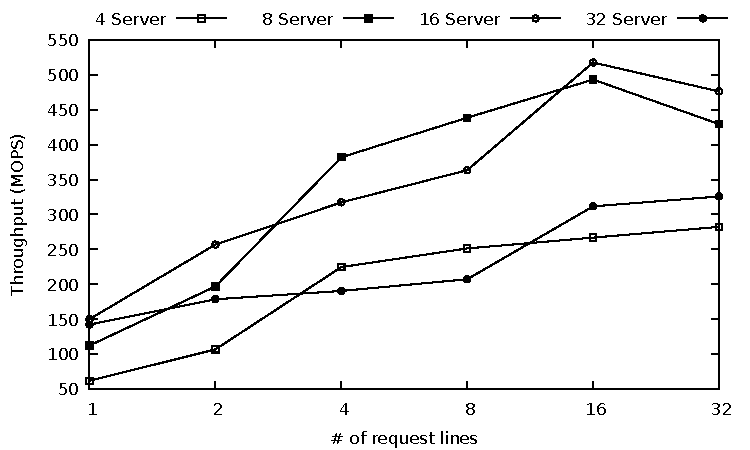
\includegraphics[width=0.9\columnwidth]{FIG/thput_by_rl.pdf}
\caption{Throughput in MOPS for a 56 thread system by number of request lines. }
\label{fig:dedicated_thput_by_rl}
\end{figure}

Correlated to the length of the queue is the number of request and response lines used to pass messages between clients and servers. \textit{Gepard} as tested in ~\autoref{eval} is configured with 4 request lines per client. \textit{Gepard}, however, manages far fewer concurrent requests due to the overhead of the fiber library. The increased rate of  request production in asynchronous dedicated delegation provides the opportunity to experiment with writing more concurrent to requests to the servers. 

~\ref{fig:dedicated_thput_by_rl} shows the measured system throughput for our benchmark with throughput plotted against the number of request lines per server-client pair. ~\ref{fig:dedicated_thput_by_rl} shows that increasing the number of request line generally increases the throughput until about 16 request lines when performance degrades. 

Do I know why?

Due to this observation we use 16 request lines for the rest of our experiments. 

\subsection{Client and Server Production Rates}
\begin{figure}[ht!]
\centering
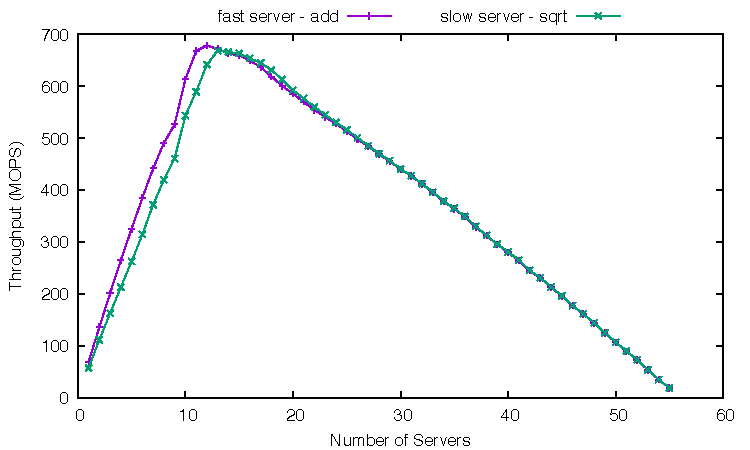
\includegraphics[width=0.9\columnwidth]{FIG/fast_and_slow_server.pdf}
\caption{Throughput in MOPS for fetch and add vs fetch and sqrt. While server speed is faster than client speed, peak throughput will require more servers when the delegated function is slower. }
\label{fig:slow_server}
\end{figure}

A feature of dedicated delegation is the ability to select the number of clients and servers operating in the system. This is a course grained way for the programmer to balance the expected request production rate of a client with the expected consumption rate of the server. In general, the programmer should increase the number of servers for more time consuming delegated functions. 

~\ref{eq:throughput} describes this rule of thumb, Where Thput\textsubscript{system} is the throughput of the entire system in MOPS, Thput\textsubscript{component} is the throughput of an individual component in MOPS, and N\textsubscript{component} is the number of that component in the system. As $Thput_{server}$ decreases, $N_{server}$ must increase to compensate until it reaches equilibrium with $N_{client} * Thput_{client}$. 

\begin{equation}
Thput_{system} = \min(N_{server} * Thput_{server}, N_{client} * Thput_{client})
\label{eq:throughput}
\end{equation}

 ~\ref{fig:slow_server} displays results of an experiment where we compare the throughput by number of servers of a faster (addition) and slower (sqrt) delegated function for our benchmark. In the regions left of peak throughput shown in  ~\ref{fig:slow_server} the system is bound by server capacity. The upward slope corresponds to the consumption rate of an individual server, or Thput\textsubscript{server}. Conversely, in the region to the right of the equilibrium point the system is bound by client production. The downward slope corresponds to the Thput\textsubscript{client}. 

~\ref{fig:slow_server} shows ~\ref{eq:throughput} to be a good model. Consumption rate slows for the server performing a more time consuming delegated function. The slower $Thput_{server}$ requires more $N_{server}$ to balance the total throughput of the clients. The peak throughput, or equilibrium point, requires more servers for the slow function than it does for the faster one, suggesting that programmers should increase the number of servers when the delegated function is more computationally intense. 

\section{Asynchronous Flat Delegation}
\begin{figure}[ht!]
\centering
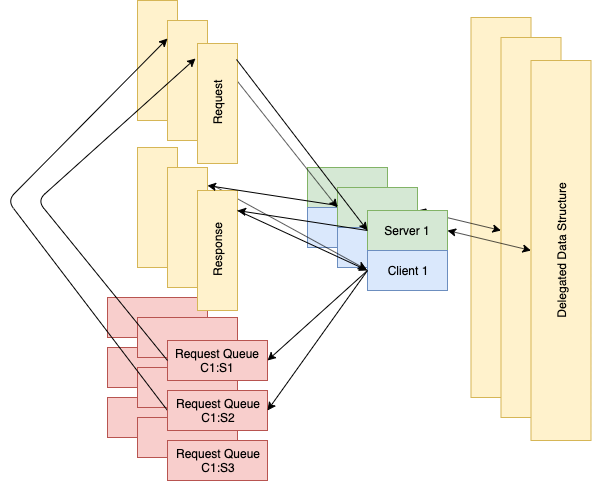
\includegraphics[width=0.9\columnwidth]{FIG/flat_async.png}
\caption{A flat delegation system with 3 client-server threads. The foreground client makes a request to itself and the background client. }
\label{fig:flat_delegation}
\end{figure}

Flat delegation combines the client and server roles of dedicated delegation into a single thread. The goal is to simplify delegation programming by finding a natural equilibrium between client and server rather than the user specified client to server ratio of dedicated delegation. ~\ref{fig:flat_delegation} sketches a sample flat delegation system with three OS threads splitting duty as client and server. Functions performing client and server duty are called from the same thread represented by the split box in the center of the figure. In ~\ref{fig:flat_delegation} the client generates requests and writes them out to the request line of the desired server, which may be the server to be invoked later on the same thread. Depending on the scheduling policy, the server function will be called to handle the requests on its request line. 

Since flat delegation does not launch dedicated server threads there is no call to \textbf{Launch\_Servers}. Besides this difference the API remains the same as dedicated delegation. 

Although the API for asynchronous flat delegation remains the same, within \textbf{Delegate\_Async()} the client must determine when to invoke the server function in addition to writing out requests. Flat delegation servers run periodically as determined by the scheduling policy instead of continuously as they do in the dedicated approach. We continued to experiment with writing requests directly to the servers as described \S\ref{pr} because of the periodic server invocation.

\subsection{Scheduling Strategies for Asynchronous Flat Delegation}  

\begin{figure}[ht!]
\centering
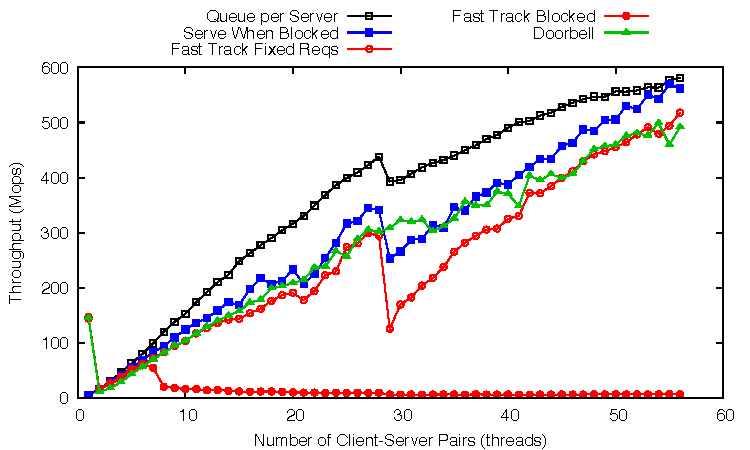
\includegraphics[width=0.9\columnwidth]{FIG/flat_delegation_strategy.pdf}
\caption{Flat delegation throughput by scheduling policy.}
\label{fig:flat_delegation_strategy}
\end{figure}

\begin{figure}[ht!]
\centering
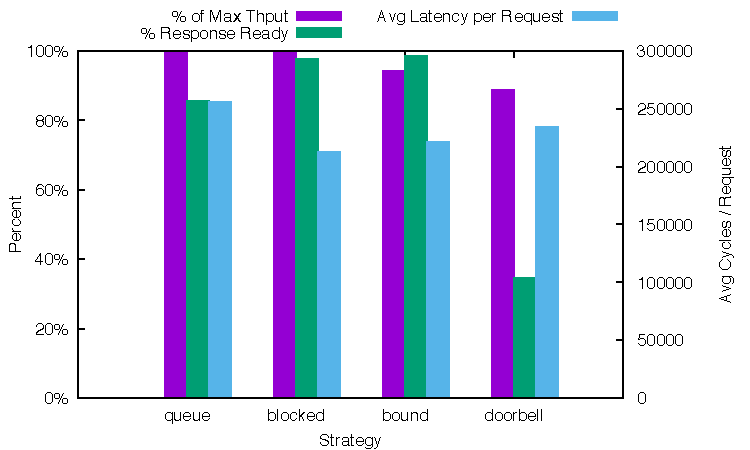
\includegraphics[width=0.9\columnwidth]{FIG/flat_latency_56.pdf}
\caption{56 server-client pair comparison of average request latency, response line availability, and comparative throughput. Greedy omitted for scale.}
\label{fig:flat_latency_56}
\end{figure}

\begin{figure}[ht!]
\centering
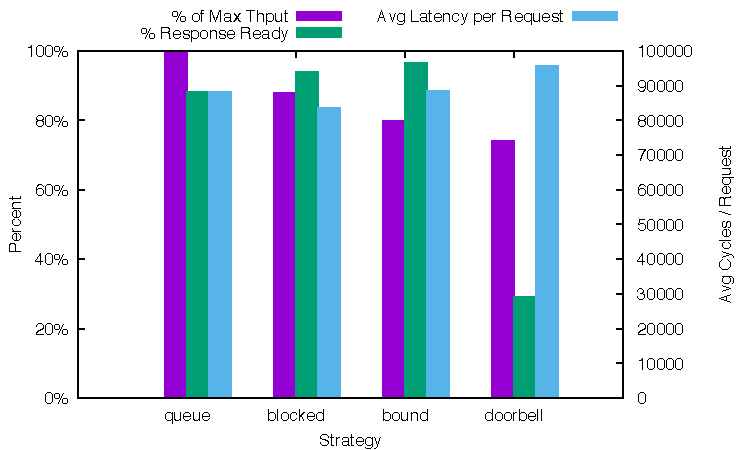
\includegraphics[width=0.9\columnwidth]{FIG/flat_latency_28.pdf}
\caption{28 server-client pair comparison of average request latency, response line availability, and comparative throughput. Greedy omitted for scale.}
\label{fig:flat_latency_28}
\end{figure}

~\ref{fig:flat_delegation_strategy} summarizes the throughput for the asynchronous flat delegation scheduling strategies tested on our benchmark. The independent variable, however represents the total number of threads running, e.g., at 20 there are 20 threads running as both client and server. The parameters for each are described in the following paragraphs. The server function is the same server function as Asynchronous Dedicated Delegation and \textit{Gepard} except it iterates through its request lines once and then returns. 

Caching requests for batch write continues to be the highest throughput (\textit{queue}), however direct request line write (\textit{blocked}) shows comparable performance for higher numbers of threads. 

~\ref{fig:flat_latency_56} and ~\ref{fig:flat_latency_28} show the average latency in clock cycles and proportion response ready when polled by delegation strategy. The Direct Write Serve When Blocked strategy shows minimum average request latency. We should note that average request latency is on the order of 10 times greater for asynchronous flat delegation than it is for asynchronous dedicated delegation shown in ~\ref{fig:saturation16RL} . 

The following subsections provide more detail on the request writing and server invocation strategies. 

\subsubsection{Pending Request Queue}

Shown as \textit{queue} in ~\ref{fig:flat_delegation_strategy} pending request queue is the same as direct delegation described in ~\autoref{pr} but with the server function invoked prior to writing and reading request lines. This approach outperformed all others in our trial, and is the approach tested in \autoref{eval}. 

\subsubsection{Direct Write Serve When Blocked}

Perhaps the simplest strategy for invoking the server function is upon a failed request issuance. After all, if the client is blocked waiting for a server to become available, the most useful thing it can do is invoke the server to handle others' requests. As shown in ~\ref{flat_delegation_strategy} \textit{blocked} shows comparable results to \textit{queue} for larger numbers of threads. \textit{Blocked} cuts down on delegation memory footprint because it eliminates the pending request queues. For larger systems, or systems with smaller amounts of on core cache \textit{blocked} may provide a way to better utilize the on core cache while maintaining higher throughput. 

The \textit{blocked} strategy exhibits a desirable property shown in ~\ref{fig:flat_latency_56} and ~\ref{fig:flat_latency_28}. The latency for any individual request, from generation to execution of the callback function is up to 15.5\% lower for \textit{blocked} than \textit{queue}. 

\subsubsection{Direct Write Fast Path, Greedy Client, Upper Bound, and Doorbell}
A proposed optimization to the serve when blocked policy was to fast track requests to a server on the same thread as the client by invoking the delegated function directly. The unintended impact of this optimization was the \textit{greedy} client problem, which is caused by victim threads attempting to write requests to the full request lines of the greedy client. The victim threads operate in server mode until the request line becomes available. However, the request line never becomes available because the greedy client's requests continue to be served by the victim threads. The greedy client problem was avoided in \textit{blocked} strategy because the client was guaranteed to invoke the server function when writes to the request lines of its own server blocked. 

To break the greedy client we experiment with an upper \textit{bound} on the client by invoking the server after a fixed number of calls to \textbf{Delegate\_Async()}. We also implement the \textit{doorbell} strategy. When a client blocks on an unavailable request line it "rings the doorbell" of the required thread by writing a 1 to its doorbell variable. Clients check their doorbell during each call to \textbf{Delegate\_Async} and invoke the server, resetting the doorbell to zero after a run of the server loop. The doorbell approach measures the highest average request latency, likely due to the latency of writing the doorbell message to a remote thread. 

\section{Ordering Guarantees}
\begin{figure}[ht!]
\centering
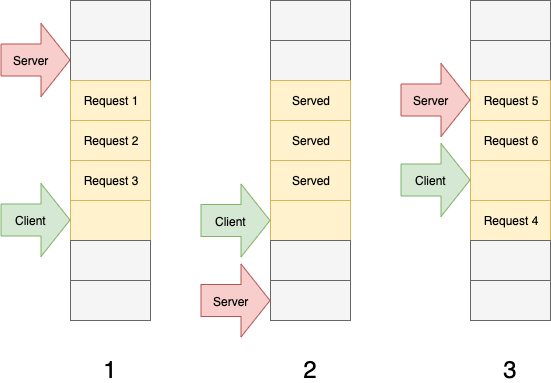
\includegraphics[width=0.9\columnwidth]{FIG/multiple_rl_race.png}
\caption{The server may execute requests out of order when multiple requests lines are used by one client. (1.) The client issues 3 requests before the server reaches its section of the request line array. (2.) The server handles all requests in this clients section before the client writes a fourth request. (3.) The client writes its next request into the next available line, after request 4 is written the next line is the first one. The requests are now executed out of order.}
\label{fig:multiple_rl_race}
\end{figure}
The asynchronous API provides no guarantee to the ordering of delegated functions. Delegated functions may be executed out of generation order when delegated to different servers because the servers are not synchronized with respect to each other. Even requests to the same server may be reordered as described below.  

Servers handle requests by iterating through all of their request lines and performing those requests with the appropriate flag. However, when there are multiple request lines per server-client pair we cannot guarantee that the requests will be performed in the order they are sent. Consider the case shown in \ref{fig:multiple_rl_race}.  A client writes a request to all but one of its request lines before the server handles the entire batch. Afterward the client writes requests to its last request line and then begins writing new requests to its first request line. Since the server handles requests in the order of the request line array, newer requests are handled before the oldest request in the last position. 

For an application with non-commutative properties, the programmer can take care to delegate the entire order critical section. It that is unfeasible, a single request line preserves the ordering of requests made by a client to a specific server, albeit with detrimental impacts to overall throughput. Experimental results are shown with both 1 and 16 request lines per client-server pair to show the difference in throughput while maintaining ordering between delegated requests to the same server. 

\chapter{Experimental Evaluation} \label{eval}
The results shown are from a 28 core, 56 thread Intel Skylake machine with 97 GB of RAM. The system has three levels of cache: On-core non-inclusive L1 and L2 of size 32KB and 1,024KB respectively, and 19,712KB of L3 cache per socket shared among the 14 physical cores on one processor. 

For spin, mutex, atomic, and flat delegation we use the number of threads available on the machine (56) unless otherwise stated. For trials with dedicated delegation \textit{async} and \textit{Gepard} we list the number of servers. The balance of remaining threads are clients.  

Like \textit{Gepard}, asynchronous delegation threads are assigned to processors in a round-robin fashion. For example, on our machine threads 0-13 are on processor 0 and 14-23 are on processor 1. Threads are assigned in the order 0, 14, 1, 15, etc... In the dedicated case all server threads are launched before any client threads. Memory for delegated data structures is allocated on the NUMA node corresponding to the processor which it is assigned. 

\section{Fetch and Add}
\begin{figure}[ht!]
\centering
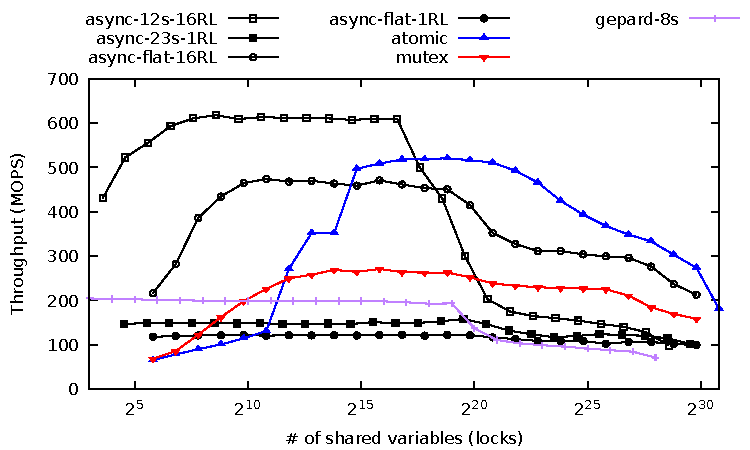
\includegraphics[width=0.9\columnwidth]{FIG/fetch_and_add_thput.pdf}
\caption{Throughput in MOPS by number of 64Byte variables. Higher is better. }
\label{fig:fetch_and_add_thput}
\end{figure}

The experiment shown in ~\ref{fig:fetch_and_add_thput} allocates a user specified number of 64B variables shown on the x-axis. OS threads are launched, and for three seconds each thread selects a variable at random and then increments that variable by its synchronization technique. After three seconds the threads are joined and the throughput in Million Operations per Second (MOPS) is reported. 

The experiment is run using the POSIX threads implementations of \textit{mutex} and \textit{spin} locks, the gcc compiler intrinsic atomic fetch and add (\textit{atomic}), and delegation approaches (\textit{Gepard-8s}, \textit{async-16s}, and \textit{async-flat}). 

The delegation approaches allocate memory as a two dimensional array, where the rows of the array are assigned to the individual server thread. \textbf{numa\_alloc\_onnode} is used to allocate the delegated data structures into dram local to the intended server's core's processor. E.g., server 1 is assigned to core 14 on processor 1, NUMA node 1. 

For flat delegation the number of shared variables is rounded up to the next highest multiple of the number of servers. For example 128 variables is rounded up to 168. For dedicated approaches when the number of shared variables is smaller than the requested number of servers the number of servers is reduced. For example a 16 server dedicated system handling 4 shared variables will run with 4 servers and 52 clients. 

The atomic and locking approaches allocate memory using \textbf{malloc} as a single array. 

\subsection{Performance Under Contention}

Delegation approaches excel for smaller numbers of shared variables. Notice dedicated delegation achieves over 600 MOPS for shared variable counts up to the size of the server cache. Flat delegation achieves consistent performance, topping out just under 500 MOPS. The reason for this even performance at low levels of shared variables is a lack of contention.

A variable is contended if multiple threads are trying to access it simultaneously. By the pigeonhole principle, we can be guaranteed that when the number of shared variables is less than the number of threads that the number of threads contending for variables is at least $ 2 * (T - V) $ where  V is total number of shared variables, and T is the number of threads. The impact of the contention is evident for the locking and atomic approaches, which demonstrate consistently low throughput until the number of shared variables increases beyond the number of threads. The probability of contention wanes as the number of variables grows. The chance that at least one pair of threads in the system is contending for a variable is described by $C = 1 - {{ V \choose T }  \over  V^{T}}$ where C is the probability of contention. C drops below 10\% at $2^{14}$ and is practically zero at $2^{19}$, which corresponds with the peak throughput of of the locking and atomic approaches. 
 
An advantage of delegation approaches, previously shown by \textit{Gepard}, is the lack of contention for variables. \ref{fig:fetch_and_add_thput} shows that asynchronous approaches meet or exceed the throughput gains made by \textit{Gepard} for small numbers of variables. 

Interestingly, asynchronous dedicated delegation outperforms all approaches on the benchmark up to $2^{20}$ shared variables. This is no accident, when the delegated data structure is sufficiently small, it remains entirely resident in the server's on-core cache. For the 16 server dedicated delegation case shown, each delegation server shares, as a hyperthread, a core with a delegation client. The combined memory overhead of delegation for the two threads is about 93 KB. This amount consumes the entire L1 cache and 62 KB of the L2 leaving 962 KB of L2 cache for the delegated data structure. 960 KB translates to (15,000) 64B variables per server, or 246,000 variables for the system. L2 cache is exhausted at 2\textsuperscript{18} variables, which is where \ref{fig:fetch_and_add_thput} shows degradation of asynchronous dedicated delegation throughput performance. 

Further, the portion of L3 cache available to the server is roughly $1 / N_{servers on processor}$ of the L3 on the processor, or 2,464 KB. This translates to 39,000 additional variables per server, or 630,000 more variables for the system. L3 is exhausted when the number of shared variables approaches 2\textsuperscript{20}. Performance continues to degrade as the number of variables resident in DRAM increases and the likelihood of cache hits decreases. 

%For quantities of shared variables smaller than the size of a single processors cache contention should be evident in L3 cache hits. More L3 cache hits indicate more contention because uncontended variables should remain in a processors exclusive L1 or L2 cache. ~\ref{fig:contention} shows delegation approaches with fewer L3 cache hits per operation compared to the atomic fetch and add and the fine grained mutex lock. 

\subsection{Memory Subsystem}

\begin{figure}[ht!]
\centering
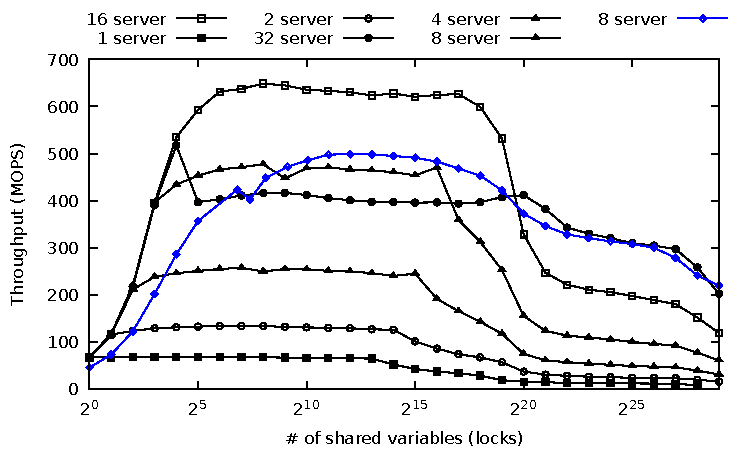
\includegraphics[width=0.9\columnwidth]{FIG/fetch_add_dedicated_vary_server.pdf}
\caption{Throughput by Shared Variables by Number of Dedicated Servers}
\label{fig:vary_server}
\end{figure}

A common theme across all approaches is the degradation of performance beginning around 2\textsuperscript{20} shared variables. Due to the randomness in the benchmark, the probability that an approach will be reading from DRAM nears 1 as the number of shared variables increases. The probability, P  that a variable picked at random in a system with cache size $S_{cache}$, variable size $S_{variable}$, total number of variables $N_{variables}$ is $P = {{S_{cache} / S_{variable}} \over N_{variables}}$. As the probability that a variable is in cache approaches zero the time to access DRAM dominates the performance of the delegation server.

Much slower access to DRAM dominates the performance of all approaches in this region, however the degradation in performance is particularly extreme for dedicated delegation because accesses are made by a smaller subset of cores. ~\ref{fig:vary_server} shows as the number of server cores increases the tail performance of dedicated delegation improves. In ~\ref{fig:ram_loads} we measure the number of loads from RAM for flat delegation vs a 16 server dedicated delegation and observe that the total number of ram loads for dedicated remains below those for flat though the RAM loads per operation scales throughout the range.  

\begin{figure}[ht!]
\centering
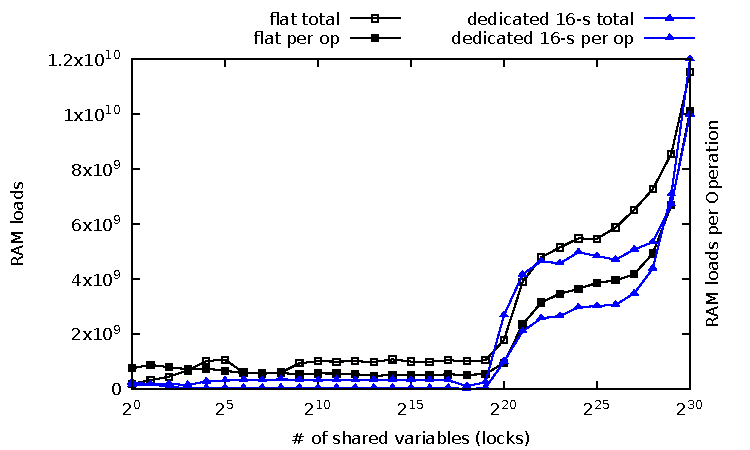
\includegraphics[width=0.9\columnwidth]{FIG/ram_accesses_by_type.pdf}
\caption{Delegation loads from RAM}
\label{fig:ram_loads}
\end{figure}

In a similar vein, a strength of flat delegation is its ability to utilize every core in the machine for DRAM access. Flat delegation also benefits from the lower cycle time for an on NUMA Node DRAM access. In comparison, the locking approaches will have a $1:N_textsubscript{NUMA Nodes} $ probability of accessing a variable at random that is addressed on the same node as the core. 


\chapter{Conclusions}
We have shown that asynchronous delegation approaches outperform the synchronous delegation approach of \textit{Gepard} on the fetch and add benchmark.  Further, asynchronous delegation can outperform fine-grained locking or atomic approaches when the delegated data structure fits within the server core's cache. Interestingly, flat delegation shows comparable performance to atomic and locking approaches as the size of the delegated data structure exceeds the size of the available cache. 



%\chapter{Some other stuff I wrote but probably shouldn't be included}
%\section{Hardware}
%Under consideration is our highly parallel machine consisting of multiple processing units, or cores, sharing resources on a single silicon processor. Cores execute threads, or sequences of machine instructions. X86 machines often support the simultaneous execution of two threads at the same time. In this hyperthreaded scenario a core's resources are shared between the threads in execution. 
%
%Processors are installed in sockets on the machine's motherboard. The processors on separate sockets communicate with each other through a bus. On a machine supporting Non Uniform Memory Access (NUMA) each socket is also a NUMA Node, with direct access to a portion of main memory (DRAM). Cores on a socket will experience greater latency accessing memory addresses on a remote NUMA node than memory addresses resident on their local NUMA node because of the time required for the data to travel across the bus. 
%
%Access to main memory is a bottleneck for modern processors, which can perform an operation in as little as 1 cycle but write to memory in the order of LOOK THIS UP. To close this latency gap processors and cores have levels of cache, small amounts of high speed memory located closer to the processing unit. Cache is typically allocated in three levels, with levels 1 and 2 dedicated to a single core, while level 3 is shared among all cores on a processor. The latency of access to levels 1, 2, and 3 is around 5, 15, 60 cycles respectively. 
%
%The cache optimization works by making a working copy of the data at a memory address and moving it into the lower latency memory closer to the core. The core can manipulate this memory locally and write it out to main memory when it is complete. When access to a memory address is predictable or frequent, data at memory addresses can be moved ahead of time, or prefetched, to the cache, and the core can benefit from the lower latency of the cache memory.   
%
%Although memory is byte addressed, the cache system manages information in 64 byte segments called cache lines. Caches are typically n-way set associative. A set can hold up to n cache lines which share a common portion of their memory address. 
%
%For example, a 32kB 8-way set associative cache has 512 cache lines split into 64 sets. Each set accepts memory addresses with bits 6-11 of the memory address in common. 
%
%When a cache is full, the least recently used cache line is evicted to a lower level cache or main memory in favor of a newer cache line. 
%
%When multiple cores access memory in the same cache line the copies resident in each core's cache may become inconsistent. Cores can snoop on another core's cache line status. If a core detects that a cache line has been modified on another core, the snooping core signals the modifying core which then forwards the modified cache line, causing an increase in access time\cite{IntelDevelopersManual}. In a concurrent program multiple cores may be writing to separate addresses resident in the same cache line. The cache line is shared between cores although the memory addresses are not. This false sharing of the memory addresses increases access latency for all cores operating on the cache line. 
%
%\section{Schemes for Shared Memory Access}
%Of course concurrent programs not only false share cache lines, they perform operations on the same memory addresses as well. Without careful synchronization by the programmer multiple cores can read and modify a memory address concurrently producing a non-deterministic result. Some of the methods for preventing this data race are described below. 
%% Locking
%Mutual Exclusion (Mutex) locks synchronize memory access through a variable that a thread must claim before moving forward with its data altering, or critical, section. When a competing thread views the lock as occupied it will wait to execute its critical section until it gets exclusive control of the lock. 
%
%There are several ways of implementing the MUTEX lock. // expand upon this.  
%
%Regardless of the implementation, synchronization schemes using locks suffer bottlenecks due to sharing the lock variable across multiple processors or sockets. In fine grained locking schemes these lock variables may take up a significant portion of memory (validate this). Additionally, memory modified in the critical section may reside in another cache, local DRAM, or another NUMA node's DRAM. 
%% Atomic Operations
%Atomic operations are those operations where 
%% Transactional Memory
%
%
%
%\chapter{Rates and System Performance}
%% Quantifying the client - server relationship
%% 



%This is how we cite a paper \cite{Farine20162243}.
%
%Below is the example of algorithm block.
%
%
%\IncMargin{1em}
%\begin{alprocedure}[!htp]
%\caption{FindFactionsAndInitiators}
%\SetKwInOut{Input}{input}\SetKwInOut{Output}{output}
%\Input{An adjacency matrix $E^*$ of dynamic network}
%\Output{ A time series of faction sets $\mathcal{F}^*$, and a time series of initiator sets $\mathcal{L}^*$ }
%\BlankLine
%\For{$i\leftarrow 1$ \KwTo $t^*$}{
%\textcolor{cyan}{\tcc*[h]{Get a matrix at time $t=i$} }
%
%$E \leftarrow E^*_{ t = i}$ \; 
%\textcolor{cyan}{\tcc*[h]{FindInitiators($E $) returns all nodes which have zero outgoing degree}}
%
%$\mathcal{L} \leftarrow$FindInitiators($E $) \;
%$\mathcal{F} = \emptyset$ \;
%\For{$l \in \mathcal{L}$}{
%\textcolor{cyan}{\tcc*[h]{FindReachNodeFrom($E,l$) returns all nodes which have any directed path to $l$}}
%
%$F_l\leftarrow$FindReachNodeFrom($E,l$) \;
%$\mathcal{F} = \mathcal{F} \cup \{F_l\}$
%}
%$\mathcal{F}^*_{t=i} = \mathcal{F}  $ and $\mathcal{L}^*_{t=i} = \mathcal{L}  $
%}
%\label{algo:FindFactionsAndInitiators}
%\end{alprocedure}\DecMargin{1em}
%
%
%The example of table is below.
%
%\begin{table}[!htp]
%\tiny
%\centering
%\caption{Table Caption1}
%\label{table:htestdes}
%\begin{tabular}{l|l|l|}
%\cline{2-3}
%                                                                                                                     & \cellcolor[HTML]{EFEFEF}\textbf{Method}                                    & \cellcolor[HTML]{EFEFEF}\textbf{Null hypothesis $H_0$}                                                                                          \\ \hline
%\multicolumn{1}{|l|}{}                                                                                               & $t$-test                                                                      & \begin{tabular}[c]{@{}l@{}}A sample has a normal distribution \\ with zero mean and unknown variance.\end{tabular}                              \\ \cline{2-3} 
%\multicolumn{1}{|l|}{}                                                                                               & \cellcolor[HTML]{EFEFEF}Sign test                                          & \cellcolor[HTML]{EFEFEF}A sample has a distribution with zero median.                                                                           \\ \cline{2-3} 
%\multicolumn{1}{|l|}{\multirow{-3}{*}{\textbf{\begin{tabular}[c]{@{}l@{}}Zero \\ mean/median \\ test\end{tabular}}}} & Wilcoxon signed rank test                                                  & A sample has a symmetric distribution around zero median.                                                                                       \\ \hline
%\multicolumn{1}{|l|}{}                                                                                               & \cellcolor[HTML]{EFEFEF}Kolmogorov-Smirnov test (KS test)                           & \cellcolor[HTML]{EFEFEF}A sample comes from a normal distribution.                                                                              \\ \cline{2-3} 
%\multicolumn{1}{|l|}{}                                                                                               & \begin{tabular}[c]{@{}l@{}}Chi-square \\ goodness-of-fit test\end{tabular} & \begin{tabular}[c]{@{}l@{}}A sample comes from a normal distribution \\ with a mean and variance estimated from a sample itself.\end{tabular}   \\ \cline{2-3} 
%\multicolumn{1}{|l|}{}                                                                                               & \cellcolor[HTML]{EFEFEF}Jarque-Bera test                                   & \cellcolor[HTML]{EFEFEF}\begin{tabular}[c]{@{}l@{}}A sample comes from a normal distribution \\ with an unknown mean and variance.\end{tabular} \\ \cline{2-3} 
%\multicolumn{1}{|l|}{\multirow{-4}{*}{\textbf{\begin{tabular}[c]{@{}l@{}}Normality \\ test\end{tabular}}}}           & Anderson-Darling test                                                      & A sample comes from a normal distribution.                                                                                                      \\ \hline
%\end{tabular}
%\end{table}
%
%
%
%\section{Support of leading faction}
%
%\begin{figure}[ht!]
%\centering
%\includegraphics[width=0.9\columnwidth]{FIG/CoorEventSup}
%\caption{An example of image in thesis }
%\label{fig:CoorEventSup}
%\end{figure}
%
%
% \appendices
% \newpage
% \appendix
%
% \chapter{Some Ancillary Stuff}
%
% Ancillary material should be put in appendices.
%
% \chapter{Some More Ancillary Stuff}
%
% Here is yet another appendix! Wahoo!

%\nocite{*}
\bibformb
\bibliography{BibFile}
\newpage
% \vita
% This is where the vita goes.  Its organization is left as an exercise.
\clearpage
    \pagestyle{pageontop}
   \thispagestyle{pageonbottom}
   %\vspace*{3in}
   \begin{large}
   \begin{center}
   {\bfseries VITA}
   \end{center}
   \end{large}
\begin{tabular}{p{2.8cm}p{10.5cm}}
NAME: & NAME LASTNAME  \\ 
    &\\
EDUCATION:  &Ph.D., Computer Science, University of Illinois at Chicago, Chicago, Illinois, 2018. \\  
            &\\
            &M.Eng., Computer Engineering, University of Illinois at Chicago, Chicago, Illinois, 20xx.\\
            &\\
            &B.Eng., Computer Engineering, University of Illinois at Chicago, Chicago, Illinois, 20xx.  \\
            &\\
ACADEMIC EXPERIENCE:  &Research Assistant, Computational Population Biology Lab, Department of Computer Science, University of Illinois at Chicago, xxxx - 2018. \\
            &\\
            &Teaching Assistant, Department of Computer Science, University of Illinois at Chicago: \\
            &\squishlist            
            \item Computer Algorithm I, Spring xxxx and  Fall xxxx.    
            \item Secure Computer Systems, Fall xxxx 
            \squishend \\
            

 \end{tabular}

\end{document}
